%\documentclass[mathserif]{beamer}
\documentclass[handout]{beamer}
%\usetheme{Goettingen}
%\usetheme{Warsaw}
\usetheme{Singapore}



%\usetheme{Frankfurt}
%\usetheme{Copenhagen}
%\usetheme{Szeged}
%\usetheme{Montpellier}
%\usetheme{CambridgeUS}
%\usecolortheme{}
%\setbeamercovered{transparent}
\usepackage[english, activeacute]{babel}
\usepackage[utf8]{inputenc}
\usepackage{amsmath, amssymb}
\usepackage{dsfont}
\usepackage{graphics}
\usepackage{cases}
\usepackage{graphicx}
\usepackage{pgf}
\usepackage{epsfig}
\usepackage{amssymb}
\usepackage{multirow}
\usepackage{amstext}
\usepackage[ruled,vlined,lined]{algorithm2e}
\usepackage{amsmath}
\usepackage{epic}
\usepackage{epsfig}
\usepackage{fontenc}
\usepackage{framed,color}
\usepackage{palatino, url, multicol}
%\algsetup{indent=2em}
\newcommand{\factorial}{\ensuremath{\mbox{\sc Factorial}}}
\newcommand{\BIGOP}[1]{\mathop{\mathchoice%
{\raise-0.22em\hbox{\huge $#1$}}%
{\raise-0.05em\hbox{\Large $#1$}}{\hbox{\large $#1$}}{#1}}}
\newcommand{\bigtimes}{\BIGOP{\times}}
\vspace{-0.5cm}
\title{A time-series classification model for Twitter opinion lexicon expansion}
\vspace{-0.5cm}
\author[Felipe Bravo Márquez]{\footnotesize
%\author{\footnotesize  
 \textcolor[rgb]{0.00,0.00,1.00}{Felipe Bravo Márquez} \\ Chief Supervisor: Associate Professor Bernhard Pfahringer \\  Supervisor: Associate Professor Eibe Frank} 

 
%\vspace{-0.3cm}
\institute{University of Waikato \\ Computer Science Department }



\date{ \today }
%\logo{\includegraphics[weight=1cm]{../img/waikato.png}}

\begin{document}
\begin{frame}
\titlepage


\end{frame}


%%%%%%%%%%%%%%%%%%%%%%%%%%%
%\section{Introduction to the Problem} 



\begin{frame}{Social Media}
\begin{scriptsize}
\begin{itemize}
 \item Microblogging services are increasingly being adopted by people in order to access and publish information.  
 \item \textbf{Twitter}: Massively used Microblogging platform where users post messages limited to 140 characters. 
 \item Twitter users tend to publish \textbf{personal opinions} regarding certain topics and news events. 
\end{itemize}
  \begin{figure}[h]
        	
\includegraphics[scale = 0.2]{pics/twitter.png}
        \end{figure}

\end{scriptsize}
\end{frame}

\begin{frame}{Opinion Mining or Sentiment Analysis}
\begin{scriptsize}\begin{itemize}
 \item Application of \textbf{NLP} and \textbf{text mining} techniques to identify and extract subjective information from textual datasets.
\end{itemize}
\pause
\begin{block}{Sentiment Classification Problem}
  \begin{enumerate}
   \item Automatically classify a textual message to classes \textcolor[rgb]{0.00,0.00,1.00}{\textbf{positive}}, \textcolor[rgb]{1.00,0.00,0.00}{\textbf{negative}}, or \textcolor[rgb]{0.00,1.00,0.00}{\textbf{neutral}}. 
  \end{enumerate} 
\end{block}

  \begin{figure}[h]
        	
\includegraphics[scale = 0.15]{pics/sent.png}
        \end{figure}


\begin{block}{Approaches}
\begin{itemize}
\item Most methods rely on opinion lexicons.
\item An opinion lexicon is a lists of terms labelled by sentiment.
\item They are normally composed of positive and negative words such as \textcolor[rgb]{0.00,0.00,1.00}{\textbf{happy}} and \textcolor[rgb]{1.00,0.00,0.00}{\textbf{sad}}.
\end{itemize}

\end{block}

\end{scriptsize}

\end{frame}


\begin{frame}{Sentiment Analysis and Social Media}
\begin{scriptsize}
\begin{itemize}
 \item Opinions are provided \textbf{freely and voluntarily} by the users in Twitter. 
 \item Analysing the sentiment underlying these opinions has important applications in product marketing and politics.
 \item The words used in Twitter include many abbreviations, acronyms, and misspelled words.
\item This words are \textbf{not} covered by most popular lexicons.
\item The manual creation of a Twitter-oriented opinion lexicon is a \textbf{time-consuming} task.

 
 
\end{itemize}

\end{scriptsize}


\end{frame}


\begin{frame}{Proposal}
\begin{scriptsize}
\begin{itemize}
\item We propose a \textbf{supervised framework} for opinion lexicon expansion for  \textbf{Twitter}.
\item Each expanded word has a \textbf{probability distribution}, describing how positive, negative, and neutral it is.
\item All the entries of the lexicon are associated with a corresponding \textbf{part-of-speech} tag.
\item This is useful for word disambiguation e.g., apple can be a company or a fruit.
\item This is the first lexical resource for Twitter with these properties. 
\item These properties are inspired by \textbf{SentiWordnet}.
\end{itemize}
\end{scriptsize}

\end{frame}


\begin{frame}{Methodology}
\begin{scriptsize}
\begin{enumerate}
\item \textbf{Collect} tweets from the domain and the time period for which the lexicon needs to be expanded. 
\item Label the collection with sentiment classes in an \textbf{automatic} way.
\item \textbf{Tag} all the words using a part-of-speech tagger.
\item Calculate word-level \textbf{time-series} for all tagged words and extract \textbf{sentiment features} from them.
\item Label the sentiment of the words that match an \textbf{existing hand-made} polarity lexicon.
\item Train a \textbf{word-level classifier} using the word-level features and the words labels from the seed lexicon.
\item Use the trained classifier to \textbf{estimate} the polarity distribution of the remaining unlabelled words.
\end{enumerate}
\end{scriptsize}
\end{frame}


\begin{frame}{Ground-Truth word polarities}
\begin{scriptsize}
\begin{itemize}
\item The expansion requires a \textbf{seed lexicon} with words labelled by sentiment.
\item We create a meta-lexicon by taking the \textbf{union} of existing hand-made lexicons.
\item We discard all words where a \textbf{polarity clash} is observed.
\end{itemize}


\begin{table}[htbp]
\begin{center}
\begin{tabular}{l|c|c|c}
\hline
 & Positive & Negative & Neutral \\ \hline
AFINN & 564 & 964 & 0 \\ 
Bing Liu & 2003 & 4782 & 0 \\ 
MPQA & 2295 & 4148 & 424 \\ 
NRC-Emo & 2312 & 3324 & 7714 \\ \hline
Union & 4331 & 7004 & 8013 \\ 
Meta-Lex & 3730 & 6368 & 7088 \\ \hline
\end{tabular}
\end{center}
\caption{Lexicon Statistics}
\label{tab:lexstats}
\end{table}
\end{scriptsize}
\end{frame}

\begin{frame}{Ground-Truth word polarities (2)}
\begin{scriptsize}
\begin{figure}[ht]
	\centering
	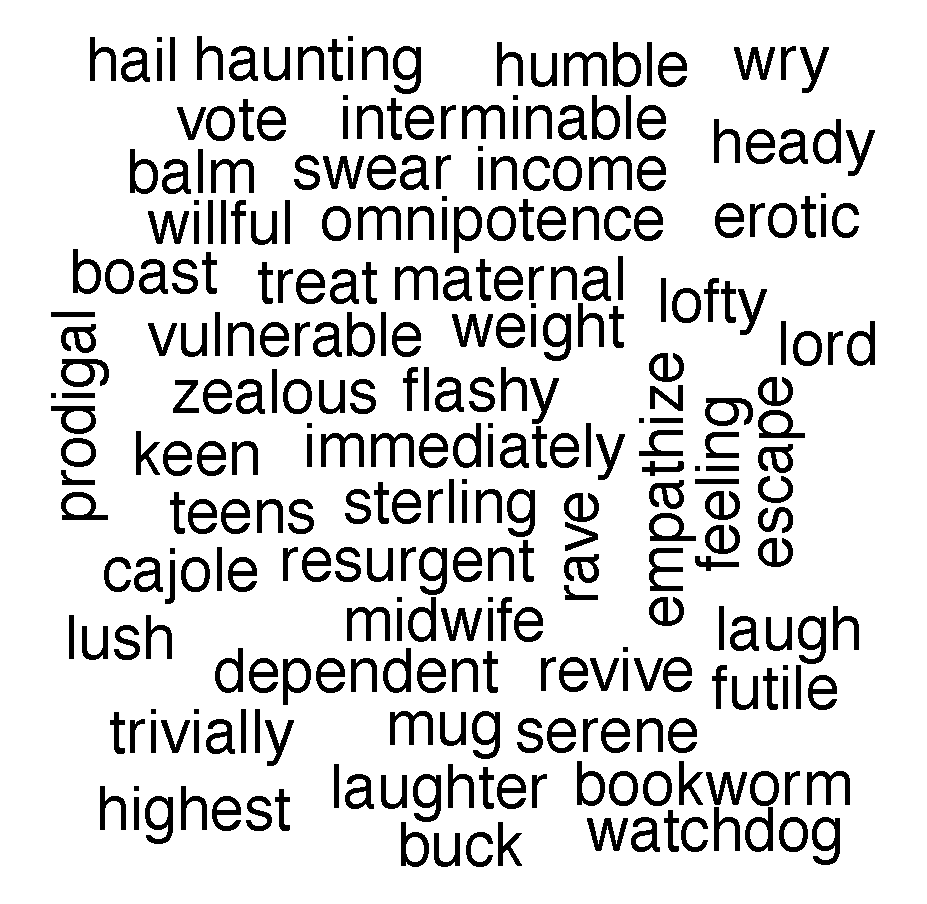
\includegraphics[scale=0.3]{../clashes.pdf}
	\caption{Polarity clashes}
	\label{fig:word_clash}
\end{figure}
\end{scriptsize}
\end{frame}




\begin{frame}{Obtaining labelled tweets}
\begin{scriptsize}
\begin{itemize}
\item We \textbf{require} a collection of time-stamped tweets with their corresponding \textbf{polarity labels}. 
\item Tweets can be collected from the Twitter API.
\item Tweets exhibiting \textbf{positive :)} and \textbf{negative :(} emoticons are labelled according to the emoticon's polarity.
\item We consider \textbf{two}  collections of tweets covering multiple topics: The \textbf{Edinburgh corpus} (ED), and the \textbf{Stanford Sentiment corpus} (STS).
\end{itemize}

\begin{table}[htbp]
\begin{center}
\begin{tabular}{l|c|c}
\hline
 & ED & STS \\ \hline
Positive & $1,813,705$ & $800,000$  \\ 
Negative & $324,917$ & $800,000$  \\ \hline
Total & $2,138,622$ & $1,600,000$ \\ 
\end{tabular}
\end{center}
\caption{Collection statistics}
\label{tab:colstats}
\end{table}
\end{scriptsize}

\end{frame}




\begin{frame}{Word-level Time-Series}
\begin{scriptsize}
\begin{itemize}
\item To train the word-level classifier we need to \textbf{calculate features} from each word found in the collection of tweets.
\item Our features exploit the \textbf{temporal structure} of the collection of labelled tweets.
\item Tweets are lowercased, tokenised and POS-tagged.

\item We prepend a \textbf{POS-tag} prefix to each word in order to differentiate \textbf{homographs} exhibiting different POS-tags.

\item We create two types of \textbf{time-series} for each word: the \textbf{Stochastic Gradient Descent} (SGD) series, and the \textbf{Semantic Orientation} (SO) series.

\end{itemize}
\end{scriptsize}

\end{frame}

\begin{frame}{The SGD time-series }
\begin{scriptsize}
\begin{itemize}
\item  This time-series is calculated by incrementally training a \textbf{linear support vector machine} from the collection of labelled tweets.
\item We use \textbf{stochastic gradient descent} (SGD) online learning process.
\begin{equation}\label{eq:sgd}
\frac{\lambda}{2}||w||^2+\sum [1- y (\mathbf{xw} +b) ]_{+}.
\end{equation}
\item The weights of this linear model correspond to POS-tagged words and are updated in an \textbf{incremental fashion}.
\item  The model's weights determine how strongly the absence or presence of a word \textbf{influences} the prediction of \textbf{polarity} classes.
\item We use \textbf{time windows} of $1,000$ examples.  

\end{itemize}
\end{scriptsize}

\end{frame}


\begin{frame}{The SO time-series }
\begin{scriptsize}
\begin{itemize}
\item  The second time-series corresponds to the \textbf{accumulated semantic orientation} (SO).
\item It is based on the \textbf{point-wise mutual information} measure.
\begin{equation}\label{eq:so}
 \operatorname{SO}(word) = log_2 \left( \frac{\operatorname{count}(\text{word $\wedge$ pos}) \times \operatorname{count}(\text{neg})}{\operatorname{count}(\text{word $\wedge$ neg}) \times \operatorname{count}(\text{pos})}\right)
\end{equation}
\item We use time windows of $1,000$ examples and the \textbf{Laplace} correction to avoid the zero-frequency problem. 


\end{itemize}
\end{scriptsize}

\end{frame}


\begin{frame}{Word-level Time-Series}
\begin{scriptsize}
\begin{figure}[htb]
\begin{center}
\begin{tabular}{c}
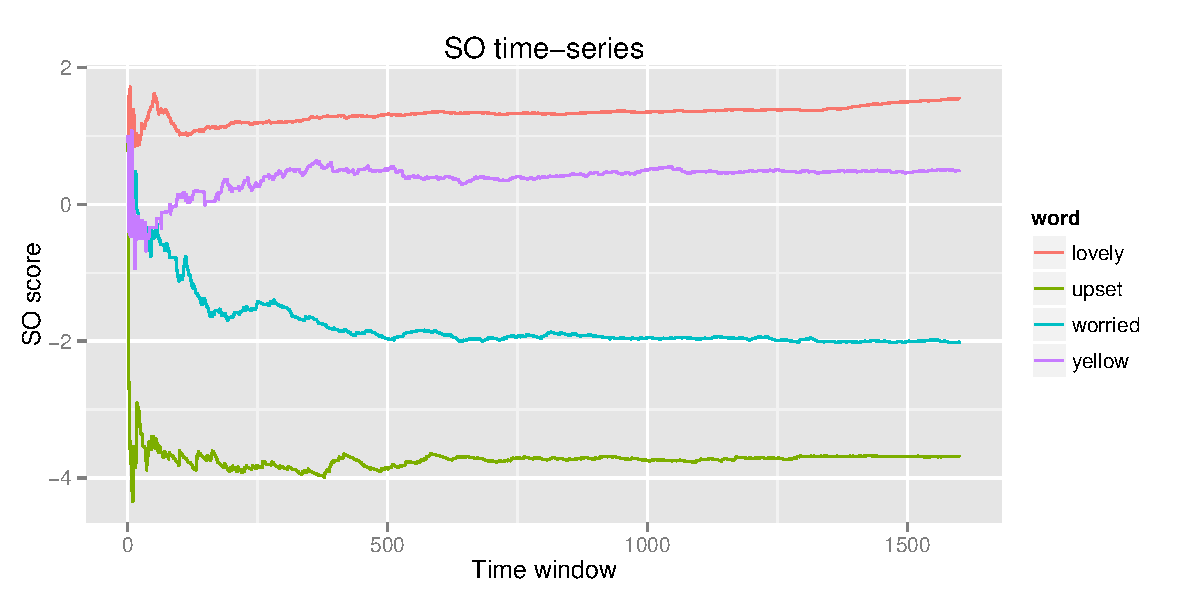
\includegraphics[scale=0.4]{../SOseries.pdf} \\
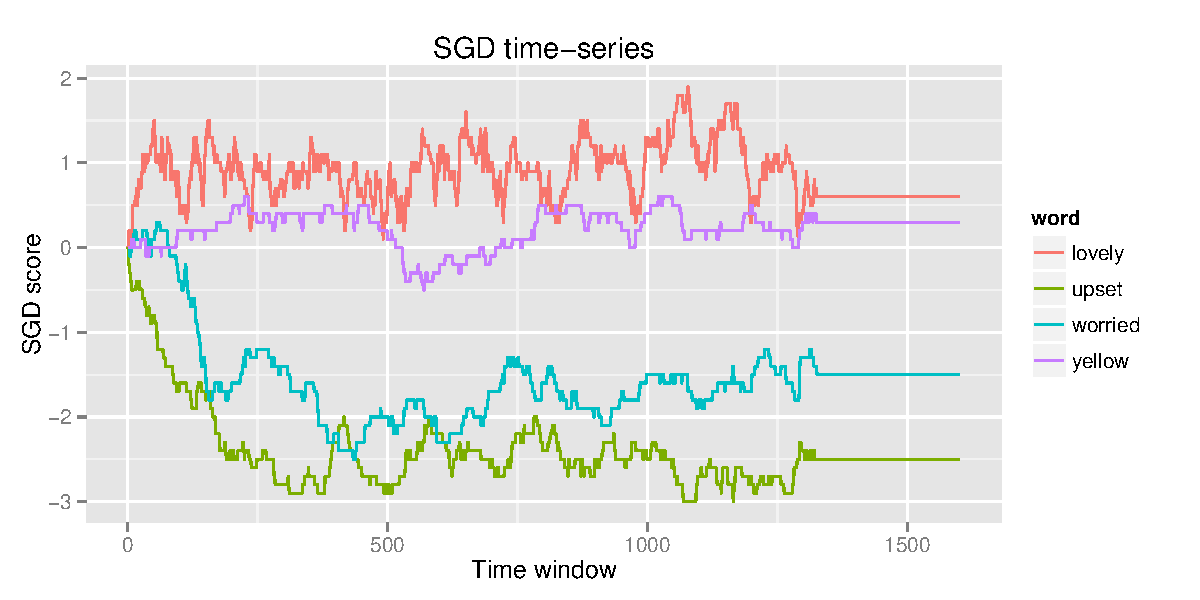
\includegraphics[scale=0.4]{../SGDseries.pdf}\\
\end{tabular}
\caption{Word-level time-series.}
\label{fig:timeseries}
\end{center}
\end{figure}
\end{scriptsize}

\end{frame}



\begin{frame}{Word-level Features}
\begin{scriptsize}
\begin{itemize}
\item We extract word-level \textbf{attributes} from both SGD and SO time-series.
\begin{table}[htbp]
\footnotesize
\begin{center}
\begin{tabular}{l|l}
\hline
Feature & Description \\ \hline
mean &  The mean of the time-series. \\ 
trunc.mean &  The truncated mean of the time-series. \\ 
median &  The median of the time-series \\ 
last.element &  The last observation of the time-series.\\ 
sd &  The standard deviation of the time-series . \\ 
iqr &  The inter-quartile range. \\ 
sg &  The fraction of times the time-series changes its sign. \\ 
sg.diff &  The sg value for the  differenced time-series. \\ \hline
\end{tabular}
\end{center}
\caption{Time-series features}
\label{tab:feat}
\end{table}

\item We also include the POS-tag of the word as a nominal attribute.

\item To create training data for machine learning, all the words \textbf{matching} the metalexicon are \textbf{labelled} according to the lexicon's polarities.

\end{itemize}
\end{scriptsize}

\end{frame}


\begin{frame}{Training data example}
\begin{scriptsize}
\begin{table}[htb]
\scriptsize
\centering
\begin{tabular}{l|llll}
  \hline
Attribute & A-lovely & A-yellow & A-upset & V-worried \\ 
  \hline
sgd.last &  0.6 &  0.3 & -2.5 & -1.5 \\ 
  sgd.mean &  0.9 &  0.2 & -2.4 & -1.6 \\ 
  sgd.trimm.mean &  0.9 &  0.2 & -2.5 & -1.6 \\ 
  sgd.median &  0.9 &  0.3 & -2.5 & -1.6 \\ 
  sgd.sd & 0.3 & 0.2 & 0.5 & 0.5 \\ 
  sgd.sg & 0.0 & 0.0 & 0.0 & 0.0 \\ 
  sgd.sg.diff & 0.2 & 0.0 & 0.1 & 0.0 \\ 
  sgd.iqr & 0.5 & 0.3 & 0.3 & 0.3 \\ 
  so.last &  1.5 &  0.5 & -3.7 & -2.0 \\ 
  so.mean &  1.3 &  0.4 & -3.7 & -1.8 \\ 
  so.trimm.mean &  1.3 &  0.4 & -3.7 & -1.9 \\ 
  so.median &  1.3 &  0.5 & -3.7 & -1.9 \\ 
  so.sd & 0.1 & 0.2 & 0.2 & 0.4 \\ 
  so.sg & 0.0 & 0.0 & 0.0& 0.0 \\ 
  so.sg.diff & 0.5 & 0.4 & 0.4 & 0.4 \\ 
  so.iqr & 0.1 & 0.1 & 0.1 & 0.1 \\ 
  pos.tag & adjective & adjective & adjective & verb \\ \hline
  label & positive & neutral & negative & negative \\ 
   \hline
\end{tabular}
\caption{Word-level feature example.}
\label{fig:featex}
\end{table}
\end{scriptsize}

\end{frame}


\begin{frame}{Feature Visualisation}
\begin{scriptsize}
\begin{figure}[htb]
	\centering
	 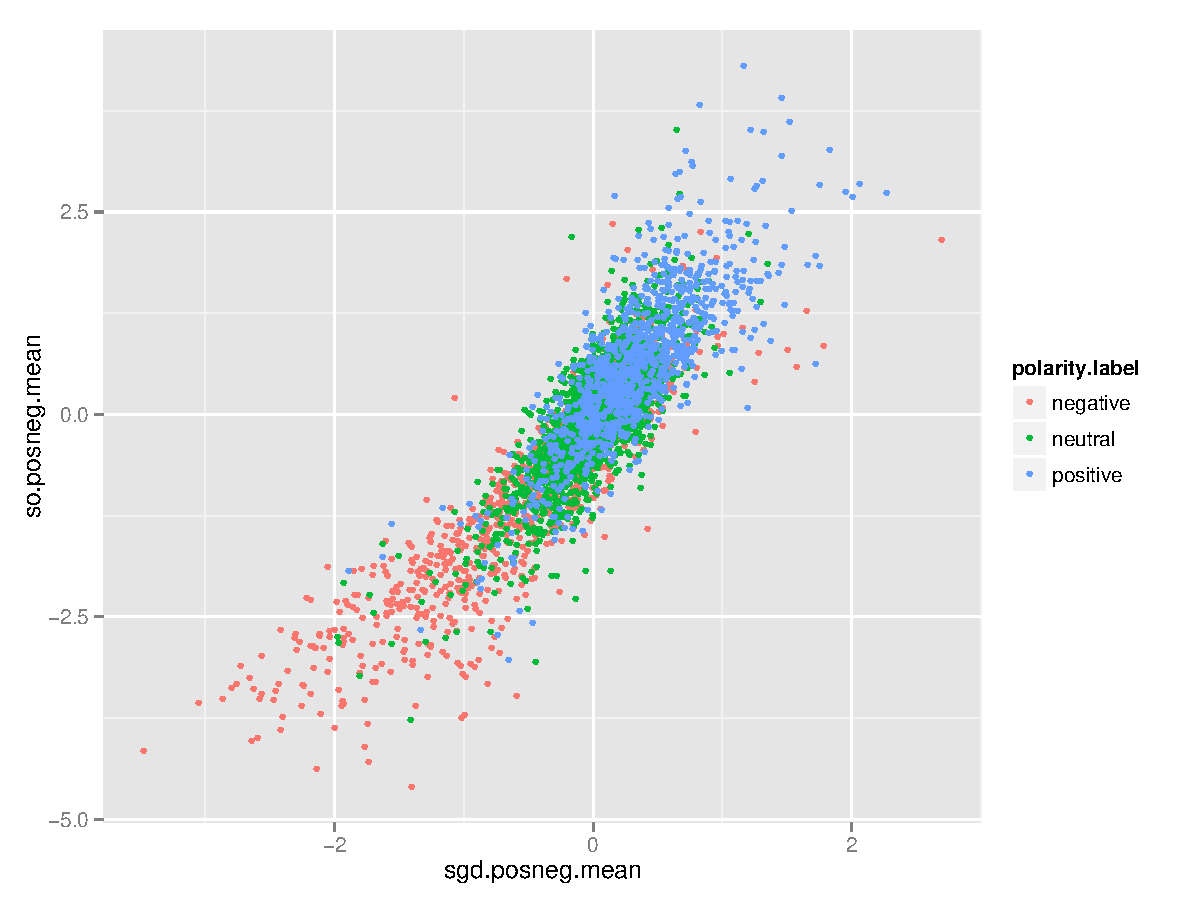
\includegraphics[width=7.5cm,height=6cm]{../SGDSO.pdf}
	\caption{SO vs SGD scatterplot.}
	\label{fig:sosgd}
\end{figure}
\end{scriptsize}

\end{frame}


\begin{frame}{Feature Visualisation (2)}
\begin{scriptsize}
\begin{figure}[ht]
\begin{center}
\begin{tabular}{c}
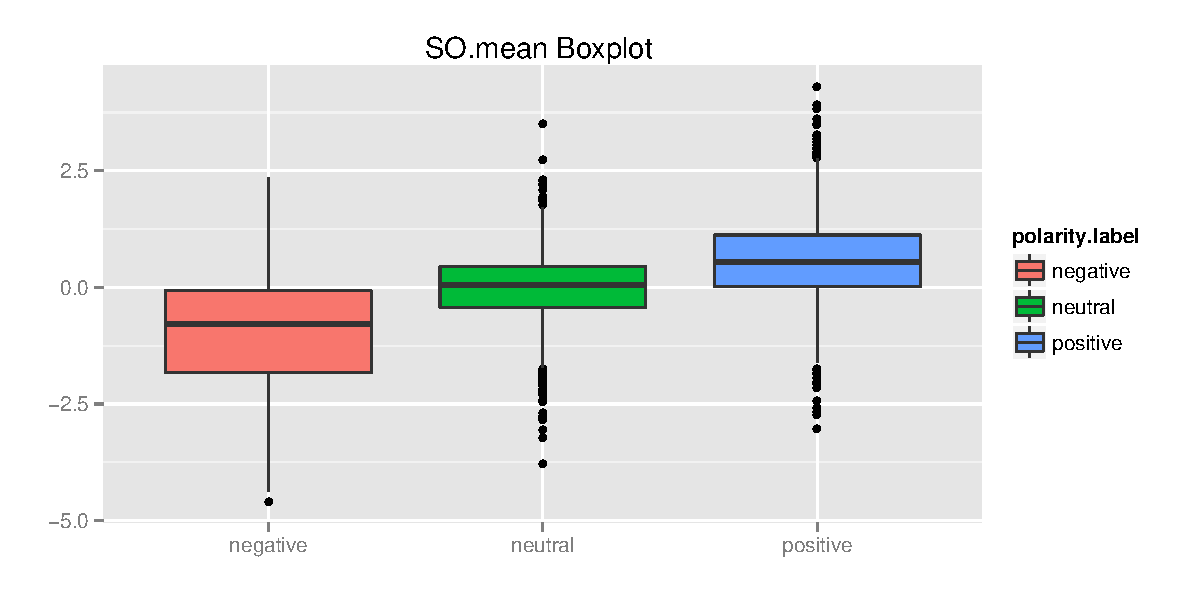
\includegraphics[scale=0.4]{../SObox.pdf}\\
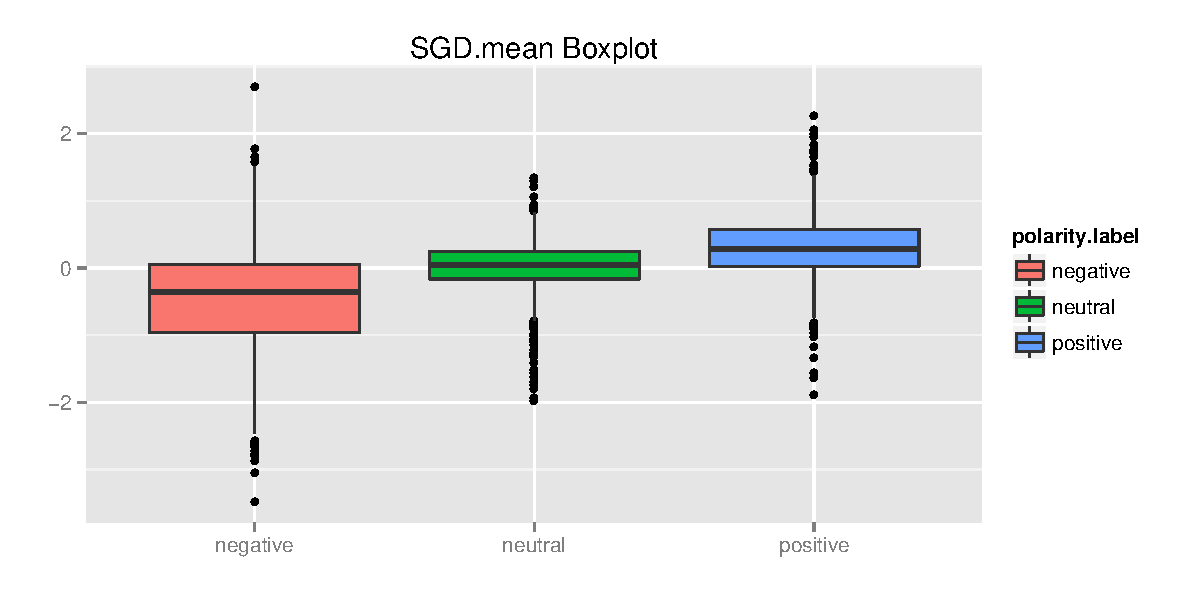
\includegraphics[scale=0.4]{../SGDbox.pdf}
\end{tabular}
\caption{SO and SGD  Boxplots.}
\label{fig:box}
\end{center}
\end{figure} 
\end{scriptsize}
\end{frame}



\begin{frame}{Word-level classification}
\begin{scriptsize}
\begin{itemize}
\item We study \textbf{three word-level} classification problems.
\item  \emph{Neutrality}: Classify words as neutral (objective) or non-neutral (subjective). 
\item \emph{PosNeg}: Classify words to positive or negative classes. 
\item \emph{Polarity}: Classify words to classes positive, negative or neutral. This is the classification problem we aim to solve. 
\item We trained \textbf{RBF SVM classifiers} for the different problems in both datasets.
\item We compare the weighted AUC obtained by \textbf{SO} with the trained classifier. 
\end{itemize}
\end{scriptsize}

\end{frame}


\begin{frame}{Word-level classification (2)}
\tiny
\begin{table}[!htb]
\begin{center}
\begin{tabular}{l|l|l|l|l|l}
\hline \hline
\multicolumn{ 6}{c}{Accuracy } \\ \hline \hline
Dataset & SO & ALL & SGD.TS+POS & SO.TS+POS & SO+POS \\ \hline
ED-Neutrality & 61.52 $\pm$ 2.21 & \textbf{65.16 $\pm$ 2.09} $\circ$ & 64.55 $\pm$ 2.27 $\circ$ & 64.9 $\pm$ 2.14  $\circ$ & 64.18 $\pm$ 2.12 $\circ$ \\ 
ED-PosNeg & 74.78 $\pm$ 2.93 & \textbf{76.04 $\pm$ 2.72} & 73.61 $\pm$ 2.51 & 75.6 $\pm$ 2.84 & 74.99 $\pm$ 2.72 \\ 
ED-Polarity & 59.48 $\pm$ 2.29 & \textbf{61.93 $\pm$ 2.1 $\circ$} & 60.97 $\pm$ 1.96 & 61.73 $\pm$ 1.98 $\circ$ & 61.57 $\pm$ 2.04 $\circ$ \\  \hline
STS-Neutrality & 62.99 $\pm$ 2.03 & \textbf{66.2 $\pm$ 2.11 $\circ$} & 65.26 $\pm$ 2.34 $\circ$ & 65.73 $\pm$ 1.98 $\circ$ & 65.77 $\pm$ 2.09 $\circ$ \\ 
STS-PosNeg & \textbf{77.18 $\pm$ 2.88} & 76.98 $\pm$ 2.82 & 75.39 $\pm$ 2.89 $\bullet$ & 76.76 $\pm$ 2.89 & 76.98 $\pm$ 2.71 \\ 
STS-Polarity & 60.2 $\pm$ 2.23 & \textbf{62.74 $\pm$ 1.52} $\circ$ & 62.34 $\pm$ 1.61 $\circ$ & 62.14 $\pm$ 1.73 $\circ$ & 62.1 $\pm$ 1.78 $\circ$ \\  \hline \hline
\multicolumn{ 6}{c}{Weighted AUC } \\ \hline \hline
Dataset & SO & ALL & SGD.TS+POS & SO.TS+POS & SO+POS \\ \hline
ED-Neutrality & 0.62 $\pm$ 0.02 &  \textbf{0.65 $\pm$ 0.02} $\circ$ & \textbf{0.65 $\pm$ 0.02} $\circ$  & \textbf{0.65 $\pm$ 0.02} $\circ$ & 0.64 $\pm$ 0.02 $\circ$ \\ 
ED-PosNeg & 0.74 $\pm$ 0.03 & \textbf{0.75 $\pm$ 0.03} & 0.71 $\pm$ 0.03 $\bullet$ & 0.74 $\pm$ 0.03 & 0.73 $\pm$ 0.03 \\ 
ED-Polarity & 0.62 $\pm$ 0.02 &  \textbf{0.65 $\pm$0.02} $\circ$ & 0.64 $\pm$ 0.02 & \textbf{0.65 $\pm$ 0.02} $\circ$ & 0.64 $\pm$ 0.02 $\circ$ \\ \hline
STS-Neutrality & 0.63 $\pm$ 0.02 & \textbf{0.67 $\pm$ 0.02} $\circ$             & 0.66 $\pm$ 0.02 $\circ$  & 0.66 $\pm$ 0.02 $\circ$ & 0.66 $\pm$ 0.02$\circ$ \\ 
STS-PosNeg & \textbf{0.77 $\pm$ 0.03} &  \textbf{0.77 $\pm$ 0.03} & 0.75 $\pm$ 0.03 $\bullet$ & \textbf{0.77 $\pm$ 0.03} & \textbf{0.77 $\pm$ 0.03} \\ 
STS-Polarity & 0.64 $\pm$ 0.02 & \textbf{0.66 $\pm$ 0.01} $\circ$  & 0.65 $\pm$ 0.02 $\bullet$  & \textbf{0.66 $\pm$ 0.02} $\circ$ & \textbf{0.66 $\pm$ 0.02} $\circ$ \\ \hline 
\end{tabular}
\end{center}
\caption{World-level classification performance.} 
\label{tab:classres}
\end{table}


\end{frame}


\begin{frame}{Expanded Lexicon}
\begin{table}[htbp]
\scriptsize
\begin{tabular}{l|l|l|r|r|r}
\hline
word & POS & label & negative & neutral& positive \\ \hline
alrighty & interjection & positive & 0.021 & 0.087 & 0.892 \\ 
boooooo & interjection & negative & 0.984 & 0.013 & 0.003 \\ 
lmaoo & interjection & positive & 0.19 & 0.338 & 0.472 \\ 
french & adjective & neutral & 0.357 & 0.358 & 0.285 \\ 
handsome & adjective & positive & 0.007 & 0.026 & 0.968 \\ 
saddest & adjective & negative & 0.998 & 0.002 & 0 \\ 
same & adjective & negative & 0.604 & 0.195 & 0.201 \\ 
anniversary & common.noun & neutral & 0.074 & 0.586 & 0.339 \\ 
tear & common.noun & negative & 0.833 & 0.124 & 0.044 \\ 
relaxing & verb & positive & 0.064 & 0.244 & 0.692 \\ 
wikipedia & proper.noun & neutral & 0.102 & 0.644 & 0.254 \\ \hline
\end{tabular}
\caption{Expanded words example.}
\label{tab:expwords}
\end{table}
\end{frame}


\begin{frame}{Expanded Lexicon (2)}
\begin{figure}[ht]
\begin{center}
\begin{tabular}{cc}
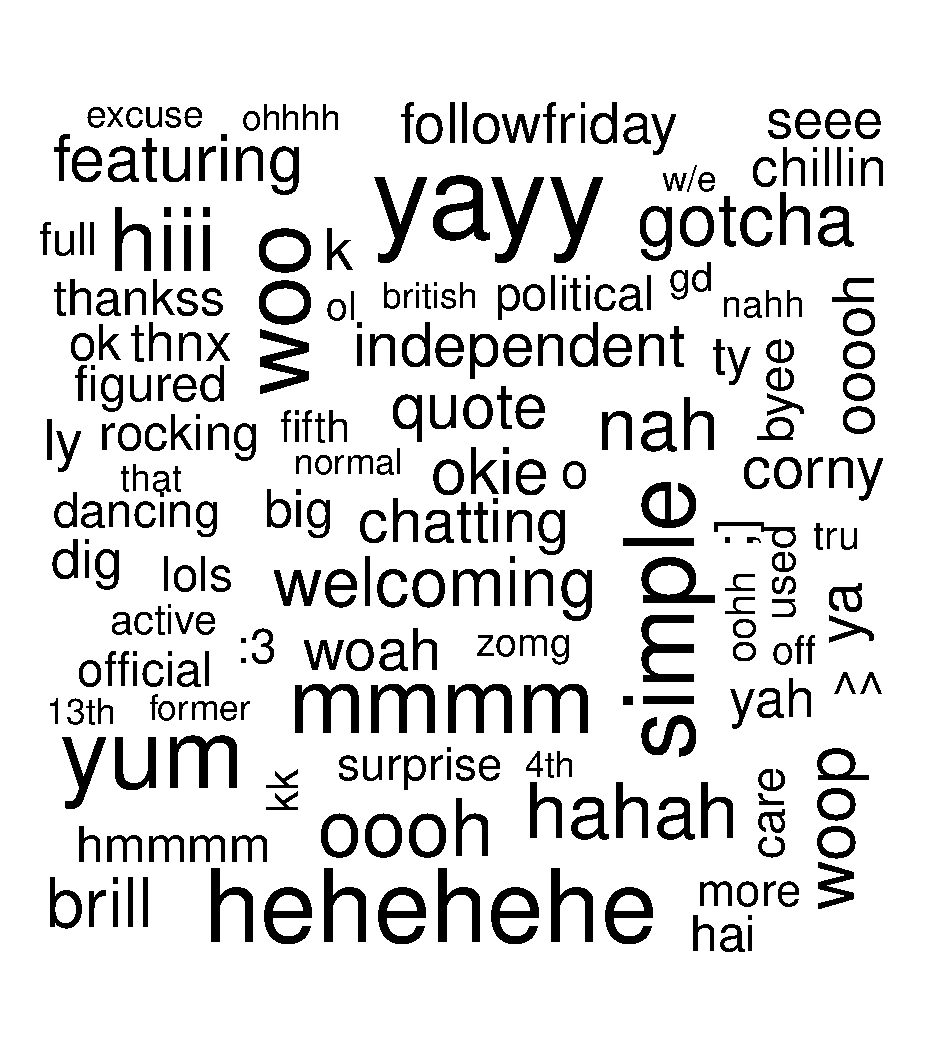
\includegraphics[scale=0.25]{../poswords.pdf}
&
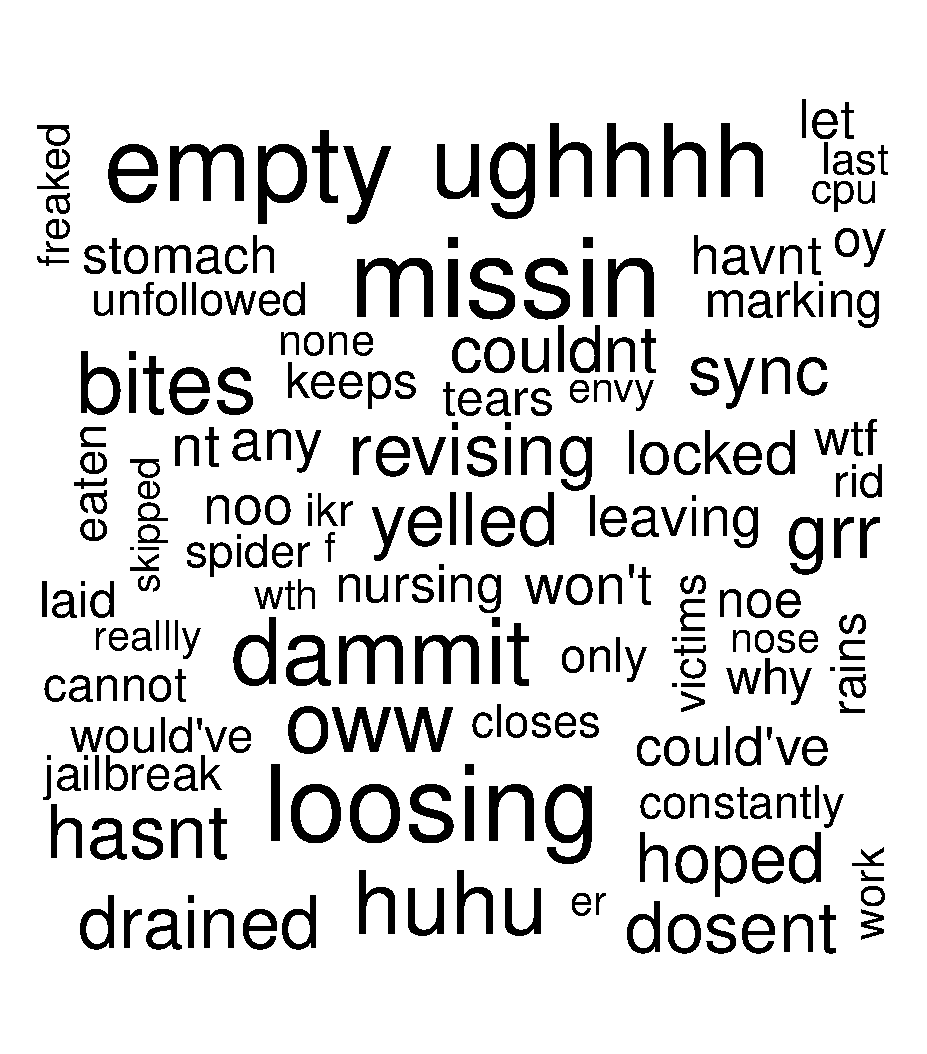
\includegraphics[scale=0.25]{../negwords.pdf}\\
(a) & (b)  
\end{tabular}
\caption{Word clouds of positive and negative words using log odds proportions.}
\label{fig:wordcloud}
\end{center}
\end{figure}
\end{frame}


\begin{frame}{Message-level classification}
\scriptsize
\begin{table}[htbp]
\begin{center}
\begin{tabular}{l|l|l|l|l}
\hline \hline
\multicolumn{ 5}{c}{Accuracy } \\ \hline \hline
Dataset & Baseline & ED & STS & Combination \\ \hline
6-coded & 71.79 $\pm$ 2.79 & 74.91 $\pm$ 2.56 $\circ$ & 75.11 $\pm$ 2.66 $\circ$ &  \textbf{75.31 $\pm$ 2.42} $\circ$ \\ 
Sanders & 71.43 $\pm$ 3.76 & 77.17 $\pm$ 3.68 $\circ$ & 77.32 $\pm$ 4.09 $\circ$ &  \textbf{77.54 $\pm$ 3.64} $\circ$ \\ 
SemEval & 76.81 $\pm$ 1.22 & 76.66 $\pm$ 1.38 & 77.7 $\pm$ 1.25 $\circ$ & \textbf{78.13 $\pm$ 1.38} $\circ$ \\ \hline \hline
\multicolumn{ 5}{c}{Weighted AUC } \\ \hline \hline
Dataset & Baseline & ED & S140 & Combination \\ \hline
6-coded & 0.77 $\pm$ 0.03 & 0.82 $\pm$ 0.03 $\circ$ & 0.82 $\pm$ 0.02 $\circ$ &  \textbf{0.83 $\pm$ 0.02} $\circ$ \\ 
Sanders & 0.77 $\pm$ 0.04 & 0.83 $\pm$ 0.04 $\circ$ & \textbf{0.84 $\pm$ 0.04} $\circ$  & \textbf{0.84 $\pm$ 0.04} $\circ$ \\ 
SemEval & 0.77 $\pm$ 0.02 & 0.81 $\pm$ 0.02 $\circ$ & \textbf{0.83 $\pm$ 0.02} $\circ$ &  \textbf{0.83 $\pm$ 0.02} $\circ$ \\ \hline
\end{tabular}
\caption{Message-level polarity classification performance.}
\label{tab:messclass}
\end{center}
\end{table}
\end{frame}


\begin{frame}{Conclusions}
\begin{scriptsize}
\begin{itemize}
\item We presented a \textbf{supervised method} for opinion lexicon expansion on \textbf{Twitter}. 
\item The method creates a lexicon with \textbf{disambiguated} POS entries and a probability distribution for \textbf{positive, negative, and neutral} classes. 
\item Sentiment analysis methods that are based on \textbf{SentiWordnet} can be easily adapted to \textbf{Twitter} by relying on our lexicon.
\item This method could be used to create \textbf{domain-specific} lexicons.
\item It could also be used to study the \textbf{dynamics} of opinion-words.

\end{itemize}
\end{scriptsize}

\end{frame}



\begin{frame}
\frametitle{Questions?}
%\vspace{1.5cm}
\begin{center}\LARGE Thanks for your Attention!\\ \end{center}

\begin{columns}
\begin{column}{0.55\textwidth}
\begin{block}{Acknowledgments}
\begin{itemize}\tiny
	\item University of Waikato Doctoral Scholarship
	\item Machine Learning Group at the University of Waikato
	
\end{itemize}
\end{block}
\end{column}
\begin{column}{0.45\textwidth}
\vspace{1.5cm}

\begin{figure}[h!]
	\centering
	\includegraphics[scale=0.3]{../../img/waikato.png}
\end{figure}
\end{column}
\end{columns}

\end{frame}




%%%%%%%%%%%%%%%%%%%%%%%%%%%

\end{document}
